%%% -*-LaTeX-*-

\chapter{Extending \TeX{} and METAFONT with floating point arithmetic}

In this chapter, we demonstrate how to incorporate another
document, such as a previously-published paper, into a
dissertation or thesis.

The University of Utah Thesis Office encourages this
practice for publications related to the thesis, with
these requirements:

\begin{itemize}

  \item
        You must have received permission to reproduce the
        document from its copyright holder, which, for
        journals is normally the journal publisher.  Such
        permissions would normally be granted on written
        request, but might take a few weeks to process, so
        plan ahead accordingly.

  \item
        A PDF file of the publication is included as
        \emph{single} chapter, with optional leading
        commentary, and suitably scaled for a maximal fit
        within the normal page boundaries (in Spring 2016,
        6.00 inches wide by 8.65 inches high).  The standard
        \LaTeX{} package \verb=pdfpages= provides the
        necessary support for inclusion of all, or part, of
        a multipage PDF file.

  \item
        The included document has its original (usually
        single) line spacing, even though most of a thesis
        uses double spacing.

  \item
        Sectional headings corresponding to the included
        PDF file must be generated for the table of
        contents.

  \item
        Even if the rest of thesis includes page headers
        with short chapter and section titles, the
        included document should have only page numbers
        at the top of each page, because the inclusion
        may already have running headers.

  \item
        Because the included document usually has its
        own bibliography, any remaining chapters that cite
        other publications must have separate bibliographies
        as well.  There is then no end-of-volume reference
        list.

\end{itemize}

Because the inclusion is a \emph{verbatim} copy of a
previously-published document, the Thesis Office accepts it
as-is, and does not proofread it, nor does it require that
it conform to the normal thesis formating rules.

Two additional packages are required in the top-level
\LaTeX{} document preamble:
%
\begin{verbatim}
\usepackage {pdfpages}            % support for multipage PDF inclusion
...
\usepackage {uuthesis-2016-f}     % usual fixups after standard packages
...
\usepackage {uuthesis-chapterbib} % support for chapter bibliographies
\end{verbatim}

The chapter might begin with some commentary on the
publication, and an acknowledgment of copyright permission.

It is followed by a setup command, then commands to generate
table-of-contents entries, using the page numbers of the
\emph{original} publication.  Those numbers are adjusted
automatically for use in the table of contents.  Finally, a
single command includes a scaled version of the document as
the contents of the rest of the chapter.  That inclusion
automatically starts on a new page.

For this sample thesis, here is what the input might look
like:
%
\begin{verbatim}
\chapter{Extending \TeX{} and METAFONT with floating point arithmetic}%
\label  {tug-paper}
...
\setupuuchapterbib

The article in this chapter was originally published in
\emph{TUGboat}, {\bf 28(3)} (2007) 501--510.  It is reproduced
here with permission of the publisher.

\uudummysection {Dedication}                              {1}
\uudummysection {Introduction}                            {1}
\uudummysection {Arithmetic in \TeX{} and METAFONT}       {1}
\uudummysection {Historical remarks}                      {1}
\uudummysection {Why no floating-point arithmetic?}       {3}
\uudummysection {IEEE 754 binary floating-point standard} {4}
\uudummysection {IEEE 754R precision and range}           {4}
\uudummysection {Remarks on floating-point arithmetic}    {5}
\uudummysection {Binary versus decimal}                   {5}
\uudummysection {Problems with IEEE 754 arithmetic}       {6}
\uudummysection {How decimal arithmetic is different}     {6}
\uudummysection {Software floating-point arithmetic}      {6}
\uudummysection {How much work is needed}                 {8}
\uudummysection {Summary}                                 {8}
\uudummysection {References}                              {8}

%%% NB: - means all pages.  Adjust scale to fit in thesis page box:
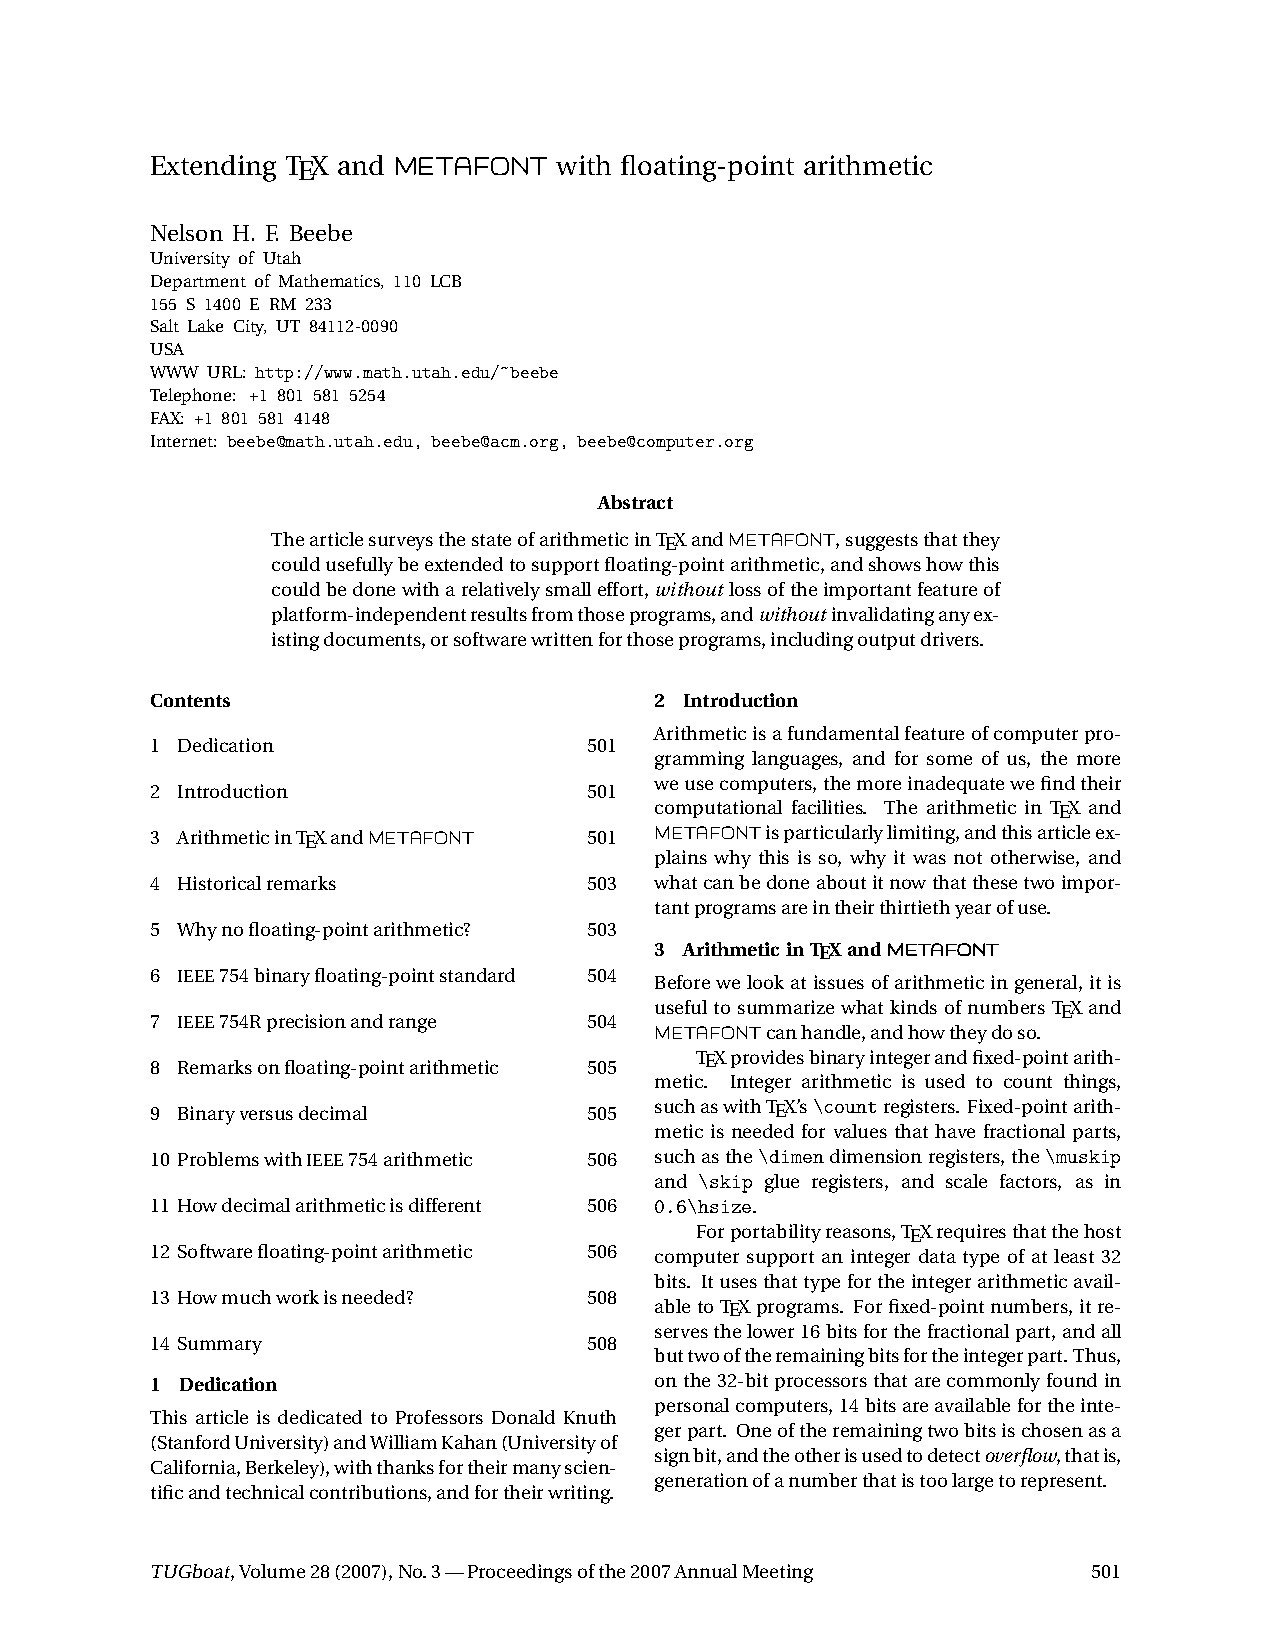
\includepdf [
                pages = -,          % want all document pages
                scale = 0.91,       % adjust to fit thesis page box
                pagecommand = {\pagestyle{plain}} % bare page numbers
            ]
            {tug2007.pdf}
\end{verbatim}
%

If the included document has subsections and subsubsections, and\slash
or figures and table, you could generate table-of-contents values for
them with additional commands like these:
%
\begin{verbatim}
\uudummysubsection    {Blah blah blah}                    {3}
\uudummysubsubsection {Blah blah blah}                    {3}
\uudummysubsubsection {Blah blah blah blah}               {4}
\uudummyfigure        {Blah blah blah blah bla}           {7}
\uudummytable         {Blah blah blah blah bla}          {10}
\end{verbatim}

However, you need not include more sectional levels than you
use for other chapters of your thesis.

At this point, we issue the block of commands above,
beginning with \verb=\setupuuchapterbib=:

\setupuuchapterbib

The article in this chapter was originally published in
\emph{TUGboat}, {\bf 28(3)} (2007) 501--510.  It is reproduced
here with permission of the publisher.

\uudummysection {Dedication}                              {1}
\uudummysection {Introduction}                            {1}
\uudummysection {Arithmetic in \TeX{} and METAFONT}       {1}
\uudummysection {Historical remarks}                      {1}
\uudummysection {Why no floating-point arithmetic?}       {3}
\uudummysection {IEEE 754 binary floating-point standard} {4}
\uudummysection {IEEE 754R precision and range}           {4}
\uudummysection {Remarks on floating-point arithmetic}    {5}
\uudummysection {Binary versus decimal}                   {5}
\uudummysection {Problems with IEEE 754 arithmetic}       {6}
\uudummysection {How decimal arithmetic is different}     {6}
\uudummysection {Software floating-point arithmetic}      {6}
\uudummysection {How much work is needed}                 {8}
\uudummysection {Summary}                                 {8}
\uudummysection {References}                              {8}

%%% NB: - means all pages.  Adjust scale to fit in thesis page box:
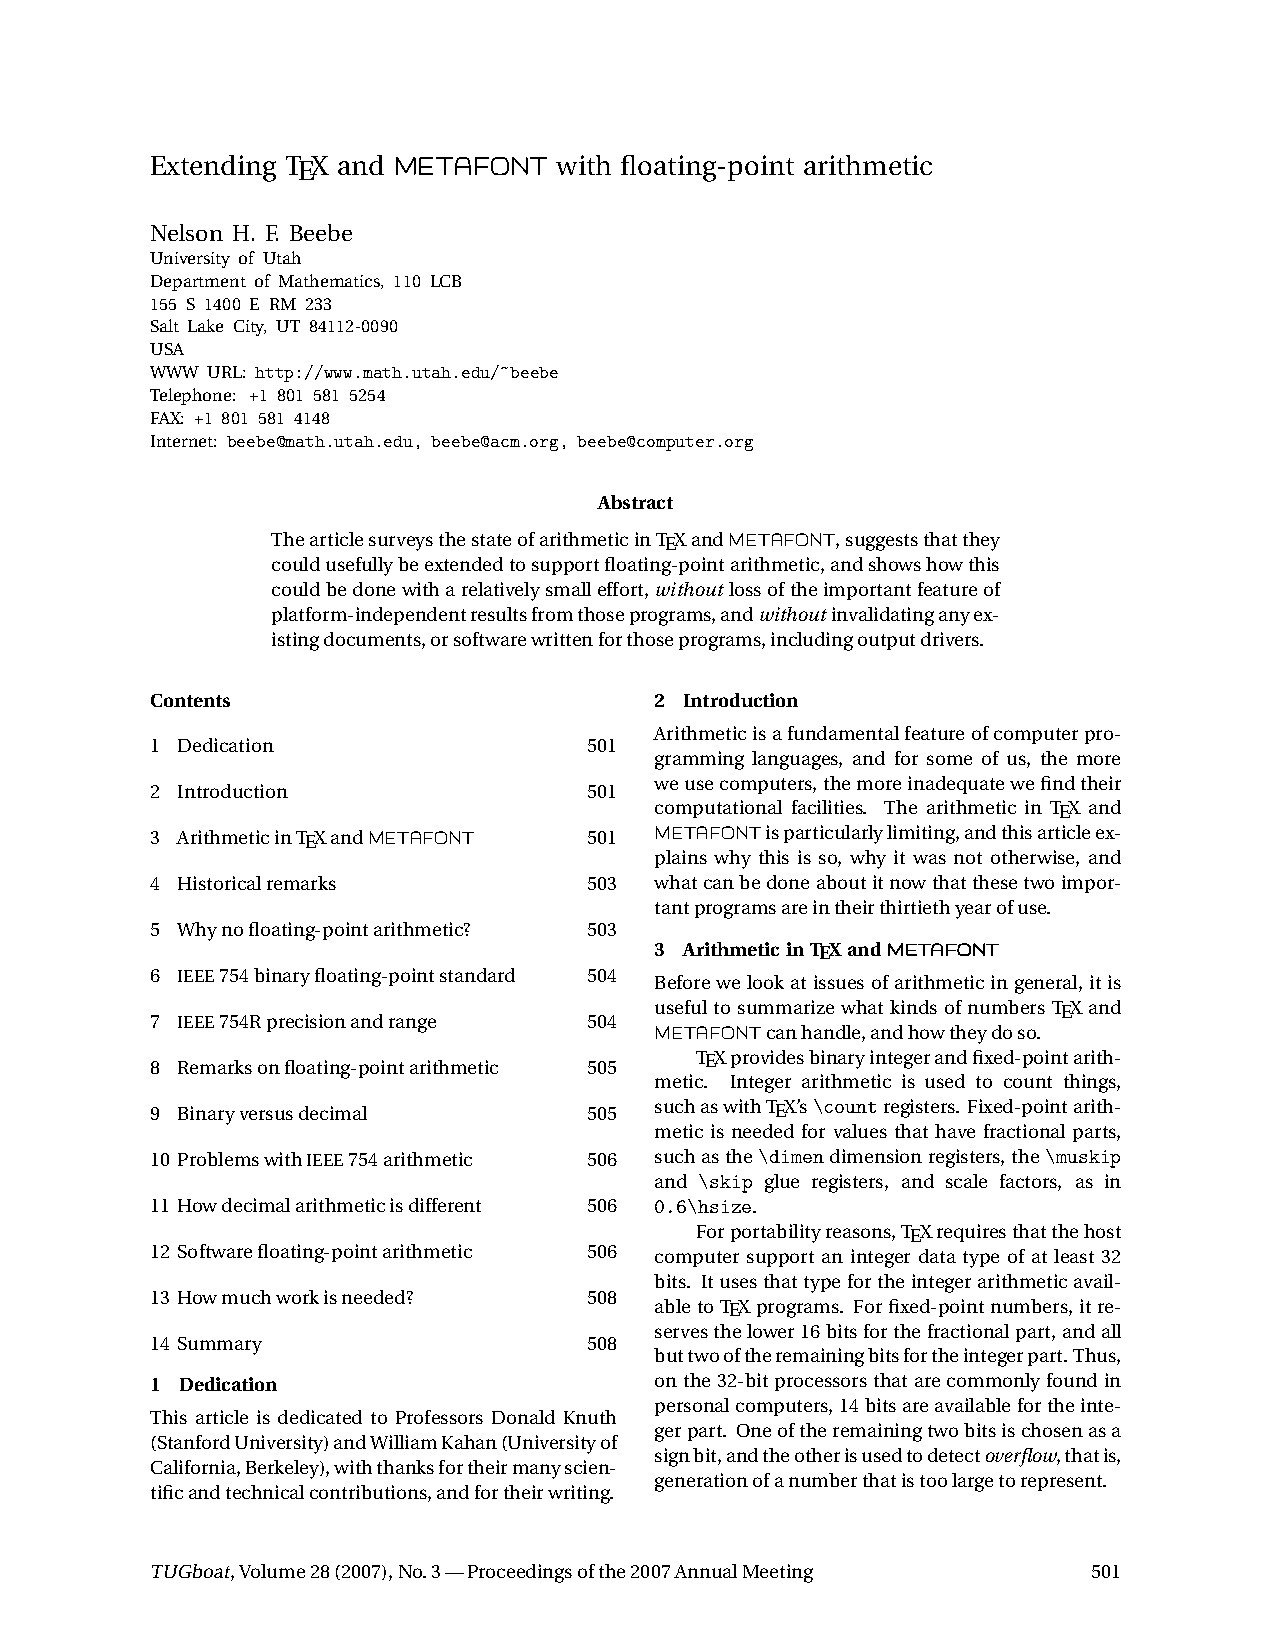
\includepdf [
                pages = -,          % want all document pages
                scale = 0.91,       % adjust to fit thesis page box
                pagecommand = {\pagestyle{plain}} % bare page numbers
            ]
            {tug2007.pdf}
